% Created 2021-12-19 Sun 10:25
\documentclass[9pt, b5paper]{article}
\usepackage[UTF8]{ctex}
\usepackage{xltxtra}
\usepackage{bera}
\usepackage[T1]{fontenc}
\usepackage[scaled]{beraserif}
\usepackage[scaled]{berasans}
\usepackage[scaled]{beramono}
\usepackage{graphicx}
\usepackage{xcolor}
\usepackage{multirow}
\usepackage{multicol}
\usepackage{float}
\usepackage{textcomp}
\usepackage{geometry}
\geometry{left=1.2cm,right=1.2cm,top=1.5cm,bottom=1.2cm}
\usepackage{algorithm}
\usepackage{algorithmic}
\usepackage{latexsym}
\usepackage{natbib}
\usepackage{minted}
\newminted{common-lisp}{fontsize=ootnotesize}
\usepackage[xetex,colorlinks=true,CJKbookmarks=true,linkcolor=blue,urlcolor=blue,menucolor=blue]{hyperref}
\author{deepwaterooo}
\date{\today}
\title{Android Study Plan}
\hypersetup{
  pdfkeywords={},
  pdfsubject={},
  pdfcreator={Emacs 27.1 (Org mode 8.2.7c)}}
\begin{document}

\maketitle
\tableofcontents


\section{View相关}
\label{sec-1}

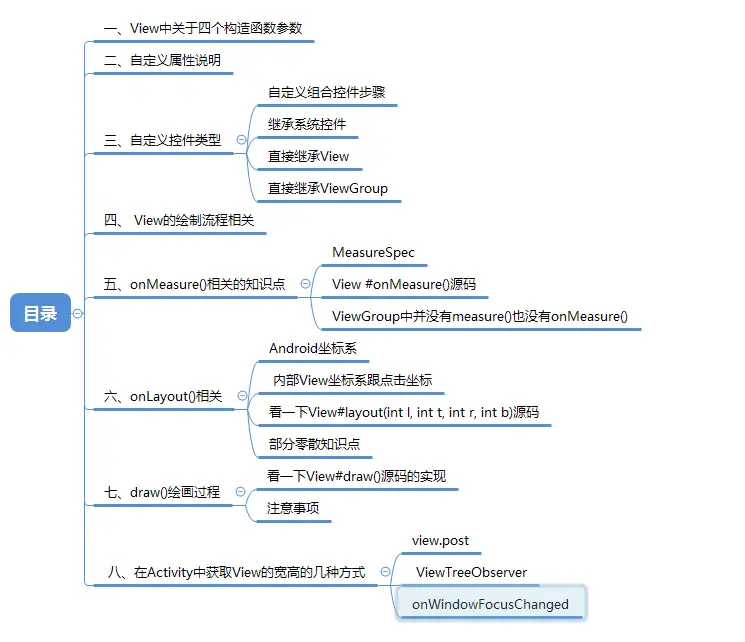
\includegraphics[width=.9\linewidth]{./pic/viewas.png}

\subsection{View 工作流程}
\label{sec-1-1}
\begin{itemize}
\item 通过 SetContentView(),调用 到PhoneWindow ,后实例DecorView ,通过 LoadXmlResourceParser() 进行IO操作 解析xml文件 通过反射 创建出View,并将View绘制在 DecorView上,这里的绘制则交给了ViewRootImpl 来完成,通过performTraversals() 触发绘制流程,performMeasure 方法获取View的尺寸,performLayout 方法获取View的位置 ,然后通过 performDraw 方法遍历View 进行绘制。
\end{itemize}
\subsection{事件分发}
\label{sec-1-2}
\begin{itemize}
\item 一个 MotionEvent 产生后,按 Activity -> Window -> DecorView(ViewGroup) -> View 顺序传递,View 传递过程就是事件分发,因为开发过程中存在事件冲突,所以需要熟悉流程:
\begin{itemize}
\item dispatchTouchEvent:用于分发事件,只要接受到点击事件就会被调用,返回结果表示是否消耗了当前事件
\item onInterceptTouchEvent:用于判断是否拦截事件(只有ViewGroup中存在),当 ViewGroup 确定要拦截事件后,该事件序列都不会再触发调用此 ViewGroup 的 onIntercept
\item onTouchEvent:用于处理事件,返回结果表示是否处理了当前事件,未处理则传递给父容器处理。(事件顺序是:OnTouchListener -> OnTouchEvent -> OnClick)
\end{itemize}
\end{itemize}
\subsection{自定义View!!}
\label{sec-1-3}
准备自定义View方面的面试最简单的方法:

就是自己动手实现几个View(由简单到复杂);
分析一些热门App中的自定义View的效果是怎么实现的;
阿里面试官: 自定义View跟绘制流程相关知识点?(标准参考解答,值得收藏)
\begin{itemize}
\item \url{https://www.cnblogs.com/Android-Alvin/p/12297933.html}
\end{itemize}

\subsection{自定义View}
\label{sec-1-4}
\subsubsection{一、View中关于四个构造函数参数}
\label{sec-1-4-1}
\begin{itemize}
\item 自定义View中View的构造函数有四个
\end{itemize}
\begin{minted}[frame=lines,fontsize=\scriptsize,linenos=false]{java}
// 主要是在java代码中生命一个View时所调用,没有任何参数,一个空的View对象
public ChildrenView(Context context) {
    super(context);
}
// 在布局文件中使用该自定义view的时候会调用到,一般会调用到该方法
public ChildrenView(Context context, AttributeSet attrs) { // AttributeSet from .xml设置
    this(context, attrs,0);
}

// 如果你不需要View随着主题变化而变化,则上面两个构造函数就可以了
// 下面两个是与主题相关的构造函数
public ChildrenView(Context context, AttributeSet attrs, int defStyleAttr) {
    this(context, attrs, defStyleAttr, 0);
}
public ChildrenView(Context context, AttributeSet attrs, int defStyleAttr, int defStyleRes) {
    super(context, attrs, defStyleAttr, defStyleRes);
}
\end{minted}
\begin{itemize}
\item 构造函数的传入参数说明
\begin{itemize}
\item context:上下文
\item AttributeSet attrs:从xml中定义的参数
\item intdefStyleAttr:主题中优先级最高的属性
\item intdefStyleRes: 优先级次之的内置于View的style(这里就是自定义View设置样式的地方)
\end{itemize}
\item 多个地方定义属性,优先级排序 Xml直接定义 > xml中style引用 > defStyleAttr>defStyleRes > theme直接定义
\end{itemize}
\subsection{二、.xml中的自定义属性}
\label{sec-1-5}
\begin{itemize}
\item 基本类型包括: integer, boolean, color, string, float, dimension, enum, flags, fraction, reference
\item 基本类型略过,其它相对重要一点儿的
\end{itemize}
\subsubsection{color :引用颜色}
\label{sec-1-5-1}
\subsubsection{dimension: 引用字体大小}
\label{sec-1-5-2}
\begin{itemize}
\item 定义
\begin{minted}[frame=lines,fontsize=\scriptsize,linenos=false]{xml}
<attr name = "text_size" format = "dimension" />
\end{minted}
\item 使用:
\end{itemize}
\begin{minted}[frame=lines,fontsize=\scriptsize,linenos=false]{xml}
<app:text_size = "28sp"  />
<app:text_size = "@android:dimen/app_icon_size" />
\end{minted}
\subsubsection{enum:枚举值}
\label{sec-1-5-3}
\begin{itemize}
\item 定义
\begin{minted}[frame=lines,fontsize=\scriptsize,linenos=false]{xml}
<attr name="orientation">
  <enum name="horizontal" value="0" />
  <enum name="vertical" value="1" />
</attr>
\end{minted}
\item 使用:
\begin{minted}[frame=lines,fontsize=\scriptsize,linenos=false]{xml}
<app:orientation = "vertical" />
\end{minted}
\end{itemize}
\subsubsection{flags:标志 (位或运行) 主要作用=可以多个值}
\label{sec-1-5-4}
\begin{itemize}
\item 定义
\begin{minted}[frame=lines,fontsize=\scriptsize,linenos=false]{xml}
<attr name="gravity">
  <flag name="top" value="0x01" />
  <flag name="bottom" value="0x02" />
  <flag name="left" value="0x04" />
  <flag name="right" value="0x08" />
  <flag name="center_vertical" value="0x16" />
</attr>
\end{minted}
\item 使用
\begin{minted}[frame=lines,fontsize=\scriptsize,linenos=false]{xml}
<app:gravity = Top|leftf />
\end{minted}
\end{itemize}
\subsubsection{raction:百分数:}
\label{sec-1-5-5}
\begin{itemize}
\item 定义:
\begin{minted}[frame=lines,fontsize=\scriptsize,linenos=false]{xml}
<attr name = "transparency" format = "fraction" />
\end{minted}
\item 使用:
\end{itemize}
\begin{minted}[frame=lines,fontsize=\scriptsize,linenos=false]{xml}
<app:transparency = "80%"  />
\end{minted}
\subsubsection{reference:参考/引用某一资源ID}
\label{sec-1-5-6}
\begin{itemize}
\item 定义:
\begin{minted}[frame=lines,fontsize=\scriptsize,linenos=false]{xml}
<attr name="leftIcon" format="reference" />
\end{minted}
\item 使用:
\begin{minted}[frame=lines,fontsize=\scriptsize,linenos=false]{xml}
<app:leftIcon = "@drawable/图片ID" />
\end{minted}
\end{itemize}
\subsubsection{混合类型:属性定义时指定多种类型值}
\label{sec-1-5-7}
\begin{itemize}
\item 属性定义
\begin{minted}[frame=lines,fontsize=\scriptsize,linenos=false]{xml}
<attr name = "background" format = "reference|color" />
\end{minted}
\item 使用
\begin{minted}[frame=lines,fontsize=\scriptsize,linenos=false]{xml}
<android:background = "@drawable/图片ID"  />
<android:background = "#FFFFFF"  />
\end{minted}
\end{itemize}
% Emacs 27.1 (Org mode 8.2.7c)
\end{document}